\section{Penelitian dan Riset Terkait}
\label{sec:riset-terkait}

\subsection{China Electronic Toll Colleciton}
China memiliki masyarakat yang sangat banyak dan setiap masyarakat memiliki sekurang kurangnya satu kendaraan. Seiring bertambah nya masyarakat di China, maka jalanan yang ada di China akan semakin penuh dengan kendaraan yang akan menghasilkan kemacetan terutama pada tol bagian pembayaran. Untuk mengatasi masalah ini China menggunakan \textit{Electronic Toll Colleciton (ETC)} yang di integrasikan dengan setiap kendaraan untuk mempercepat proses ini \parencite{penelitianterkait1}.

China menggunakan KubeEdge untuk melakukan proses \textit{deployment} \textit{ETC} untuk 100,000 \textit{nodes} dengan total 500,000 aplikasi yang diluncurkan menggunakan KubeEdge tersebar untuk 29 dari 34 provinsi. Proses \textit{deployment} dilakukan secara otomatis dengan membuat sistem \textit{workflow engine} pada kubernetes sehingga proses \textit{deployment} dapat dilakukan dengan cepat dan mudah. Dengan menggunakan metode ini sistem pembayaran tol di China menjadi 10x lebih cepat dari sebelumnya \parencite{penelitianterkait1}.

\begin{figure}[h]
  \centering
  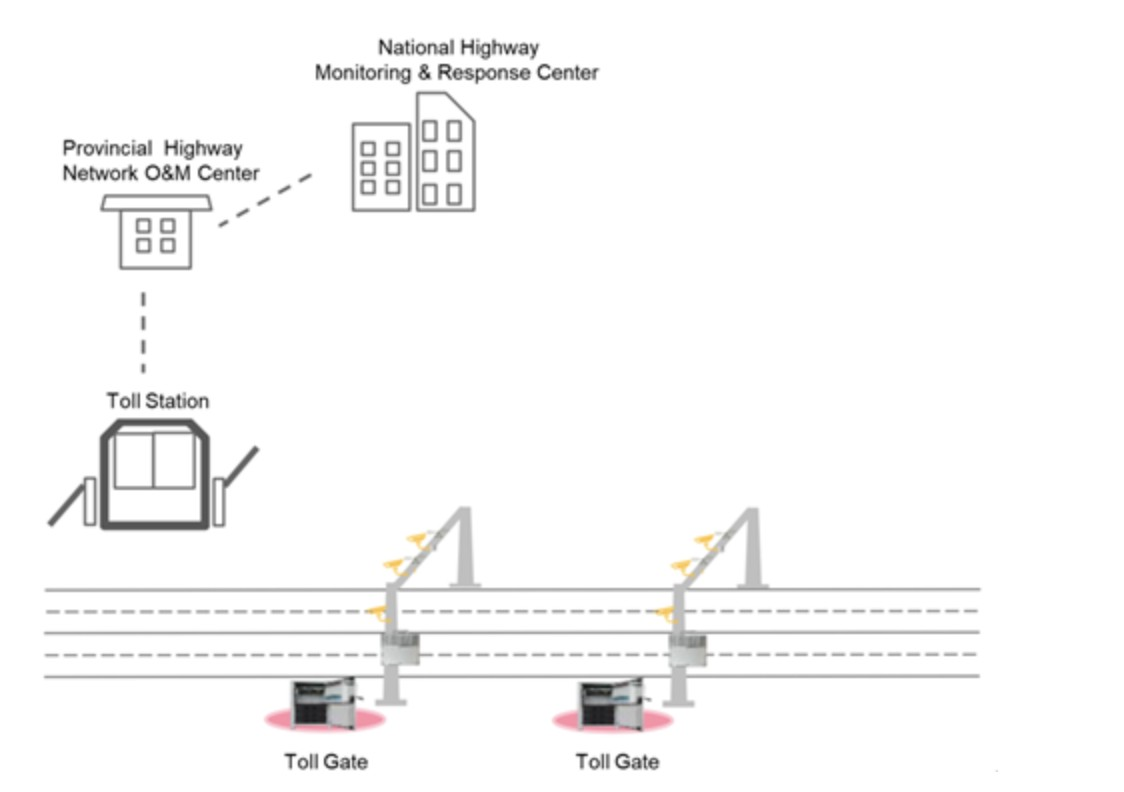
\includegraphics[width=0.8\textwidth]{resources/chapter-2/china-highways.jpg}
  \caption{Implementasi sistem \textit{ETC} di China \parencite{penelitianterkait1}}
  \label{fig:china-highways}
\end{figure}

\begin{figure}[h]
  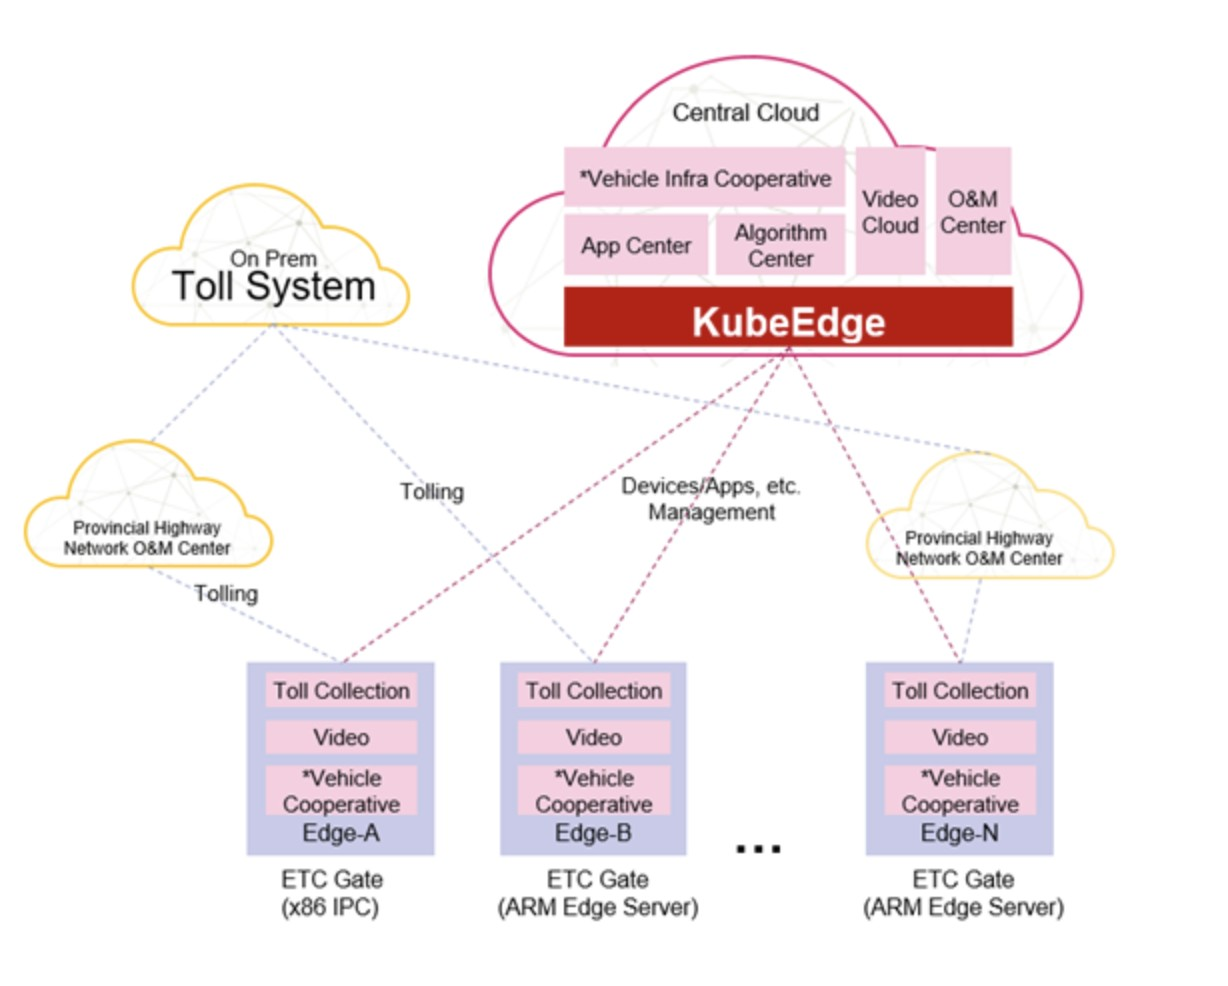
\includegraphics[width=0.8\textwidth]{resources/chapter-2/arsitektur-china-highways.jpg}
  \caption{Arsitektur sistem \textit{ETC} di China \parencite{penelitianterkait1}}
  \label{fig:architecture-china-highways}
\end{figure}

\subsection{A Model for the Remote Deployment, Update, and Safe Recovery for Commercial Sensor-Based IoT Systems}
Penelitian ini menggali tantangan-tantangan khusus terkait infrastruktur yang didedikasikan untuk penyebaran dan manajemen aplikasi secara jarak jauh. Penelitain ini membahas tantangan-tantangan manajemen terkait sistem sensor \textit{IoT}, dan mengusulkan sebuah cara serta metodologi untuk mengatasi hal tersebut.

Penelitian ini mengimplementasikan solusi sebagai sistem infrastruktur perangkat lunak untuk produk IoT bisnis yang lengkap. Penelitian ini melakukan \textit{deployment} pada 100 perangkat penjual minuman yang tersebar di tiga lokasi. Setiap perangkat bergantung pada sensor yang memantau statusnya dan pada \textit{gateway} yang mengendalikan perilakunya.

\begin{figure}[h]
  \centering
  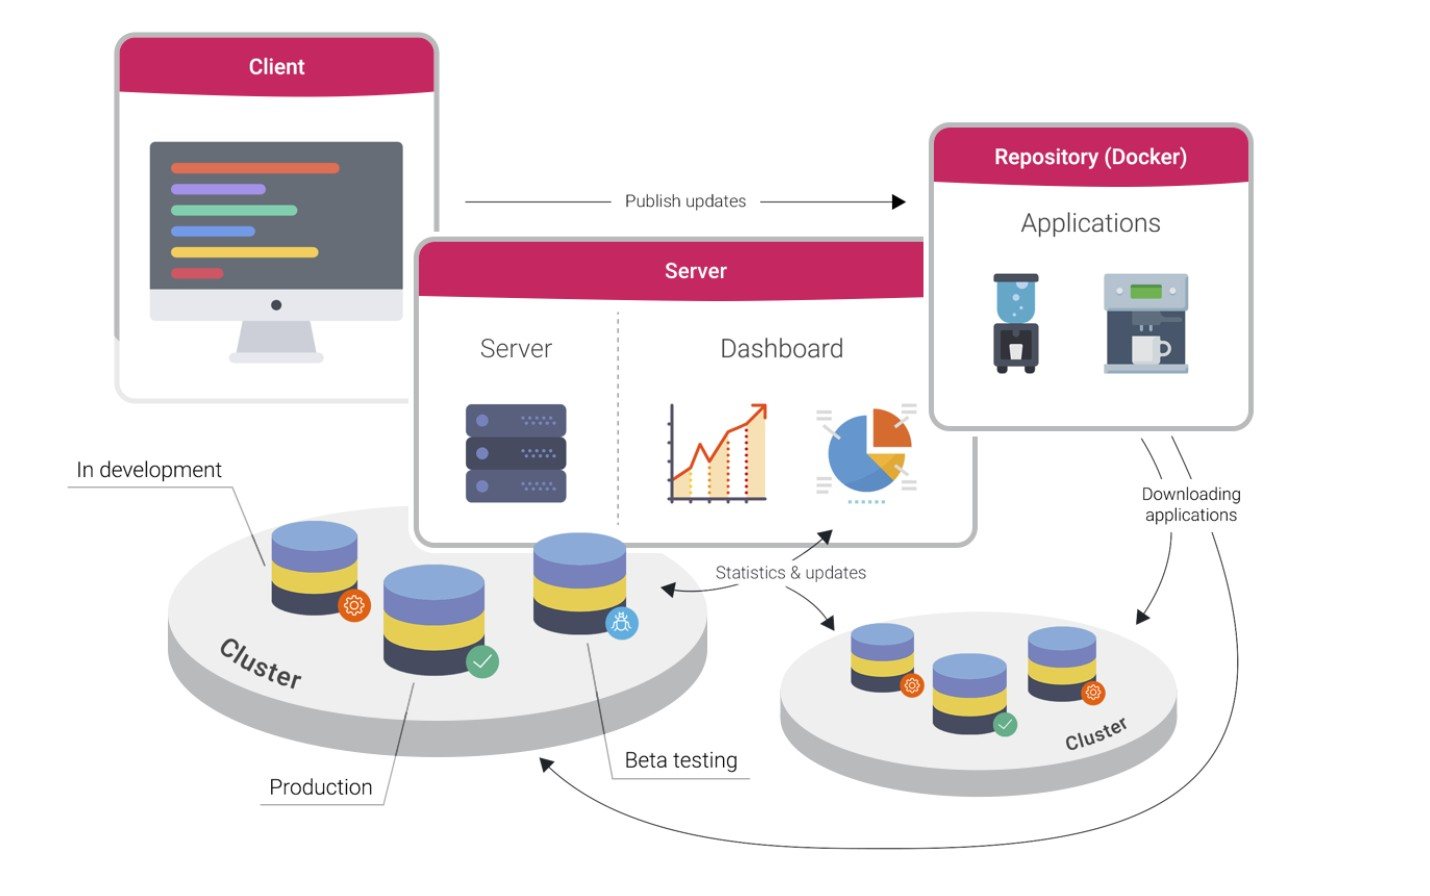
\includegraphics[width=0.8\textwidth]{resources/chapter-2/arsitektur-remote-deployment.jpg}
  \caption{Arsitektur remote \textit{deployment} \parencite{RemoteDeployment}}
  \label{fig:architecture-remote-deployments}
\end{figure}

Selama penelitian ini berlangsung, penelitian ini berhasil menerima 133 \textit{update} pada pernagkat \textit{IoT} Selain itu, 80\% perangkat beroperasi tanpa gangguan selama 250 hari, dengan 20\% mengalami kegagalan akibat faktor eksternal; dari 80\% tersebut, 30\% mengalami kegagalan pembaruan sementara akibat kapabilitas perangkat yang berkurang dan sistem dengan berhasil melakukan pemulihan otomatis dalam 100\% kegagalan sementara tersebut \parencite{RemoteDeployment}.

Solusi yang dibuat penelitian ini mengandlakan keamanan serta \textit{failsafe} yang dapat melakukan \textit{remote deployment} dengan baik serta aman sehingga dapat mendeteksi kegagalan yang terjadi pada perangkat dan melakukan \textit{recovery} dengan cepat. Berikut merupakan beberapa cara untuk melakukan \textit{remote deployment} atau seringkali disebut sebagai OTA \textit{(Over the air)}.


\begin{figure}[h]
  \centering
  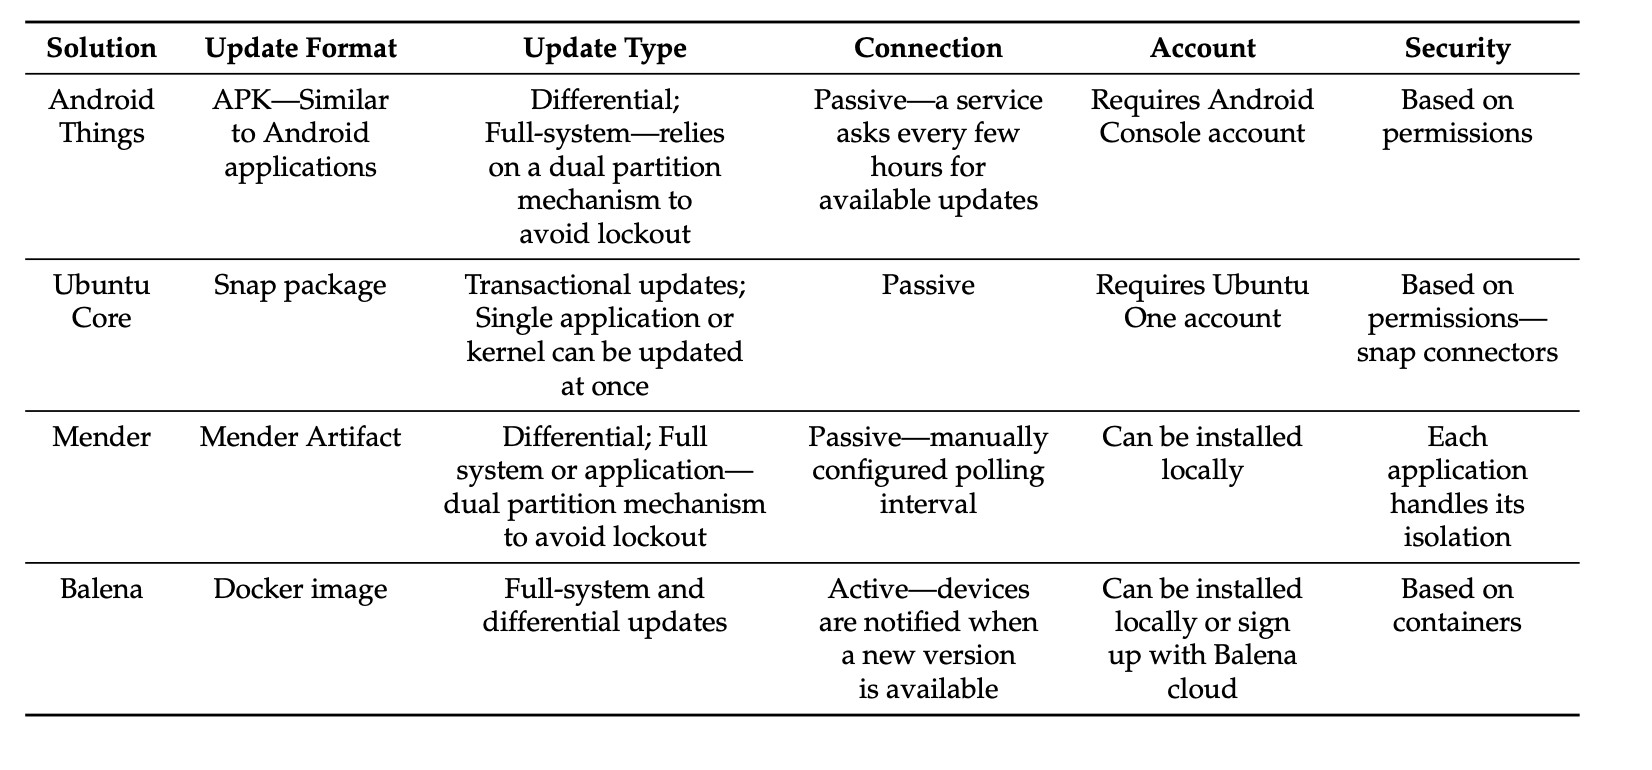
\includegraphics[width=0.8\textwidth]{resources/chapter-2/perbandingan-remote-deployment.jpg}
  \caption{Perbandingan tata cara \textit{remote deployment} \parencite{RemoteDeployment}}
  \label{fig:comparison-remote-deployments}
\end{figure}

Dapat dilihat dari gambar tersebut bahwa terdapat berbagai solusi untuk berbagai tipe \textit{remote deployment}. Pada kasus ini dapat dibuat suatu cara yang mengadopsi update type serta koneksi dari keempat tipe tersebut. Perangkat akan melakukan \textit{polling} kepada \textit{server} untuk mengecek apakah terdapat versi terbaru atau tidak. Selain itu dari sisi \textit{Server} juga dapat membuat suatu notifikasi yang dapat diterima oleh perangkat jika terdapat \textit{update} baru yang siap digunakan.


\subsection{Device discovery strategies for the IoT}
Paper ini membahas tantangan \textit{device discovery} dalam jaringan Internet of Things (IoT). Fokus utama penelitian ini yaitu pada topologi jaringan dan bagaimana topologi jaringan mempengaruhi proses \textit{device discovery}. Tiga topologi jaringan yang dievaluasi adalah terpusat, terdesentralisasi, dan hirarkis, dengan kriteria evaluasi mencakup storage yang dibutuhkan, waktu \textit{discovery}, \textit{traffic} jaringan, persentasi sukses dan \textit{reliability}

\textit{Device discovery} adalah proses penting untuk mengidentifikasi dan memanfaatkan perangkat sesuai kebutuhan. Strategi yang diusulkan dalam penelitian ini berfokus pada peningkatan efisiensi dalam menemukan perangkat melalui topologi jaringan yang berbeda. Simulasi multi-agen digunakan untuk menganalisis dampak perubahan topologi dalam proses penemuan. Hasil simulasi menunjukkan bahwa topologi terpusat cenderung lebih efisien dalam hal komunikasi karena menggunakan satu pesan untuk proses \textit{device discovery}, sedangkan topologi terdesentralisasi dan hirarkis memerlukan penyebaran pesan yang lebih luas. Namun, topologi terpusat kurang efisien dalam hal penyimpanan karena semua data terpusat pada node pusat sehingga memerlukan \textit{storage} yang lebih besar \parencite{DeviceDiscovery}.

\begin{figure}[h]
  \centering
  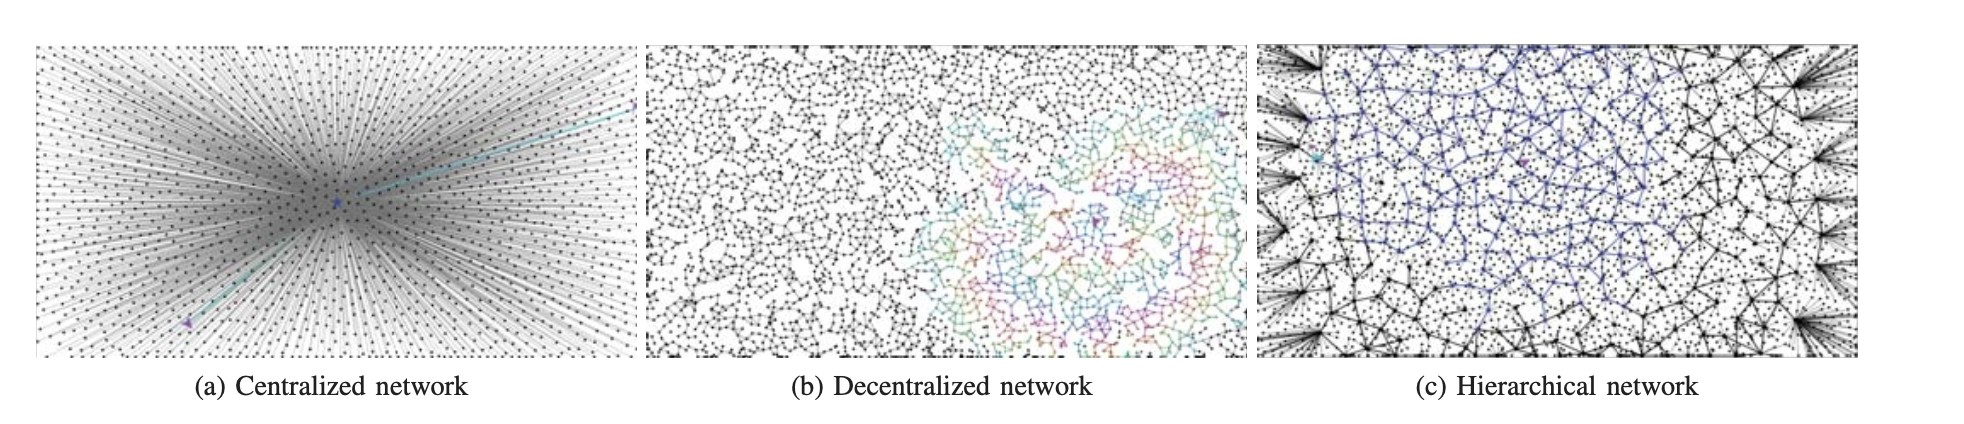
\includegraphics[width=1\textwidth]{resources/chapter-2/penelitian-terkait-device-discovery-strategy.jpg}
  \caption{Hasil penelitian topologi jaringan pada proses \textit{device discovery} \parencite{DeviceDiscovery}}
  \label{fig:stragey-for-device-discovery}
\end{figure}

